
\section{Perspectivas de mejora}

Como hemos podido comprobar los resultados no son satisfactorios, ya que según nuestro modelo el experimento no será capaz de inferir ningún tipo de resultado a partir de las medidas con los silicios. La solución la encontramos en la TPC. La TPC nos permite recuperar estadística a partir de un \textit{trigger} interno llamado L1 basado en la multiplicidad de los pads de lectura, esto es, en el número de electrones que llega a cada uno de los pads.

Para que sean medidos satisfactoriamente por este \textit{trigger} L1 necesitamos que los tritios se frenen completamente en la cámara de deriva, en la caja de $295 \times 295 \times 255 $ mm$^{3}$. No es difícil calcular cuantas partículas se frenan en la cámara, solo tenemos que calcular el \textit{punch-trought} (distancia máxima que alcanza) de la partícula en el gas, proyectarla en la dirección de la partícula y ver si no se sale. 

\begin{figure}[H] \centering
    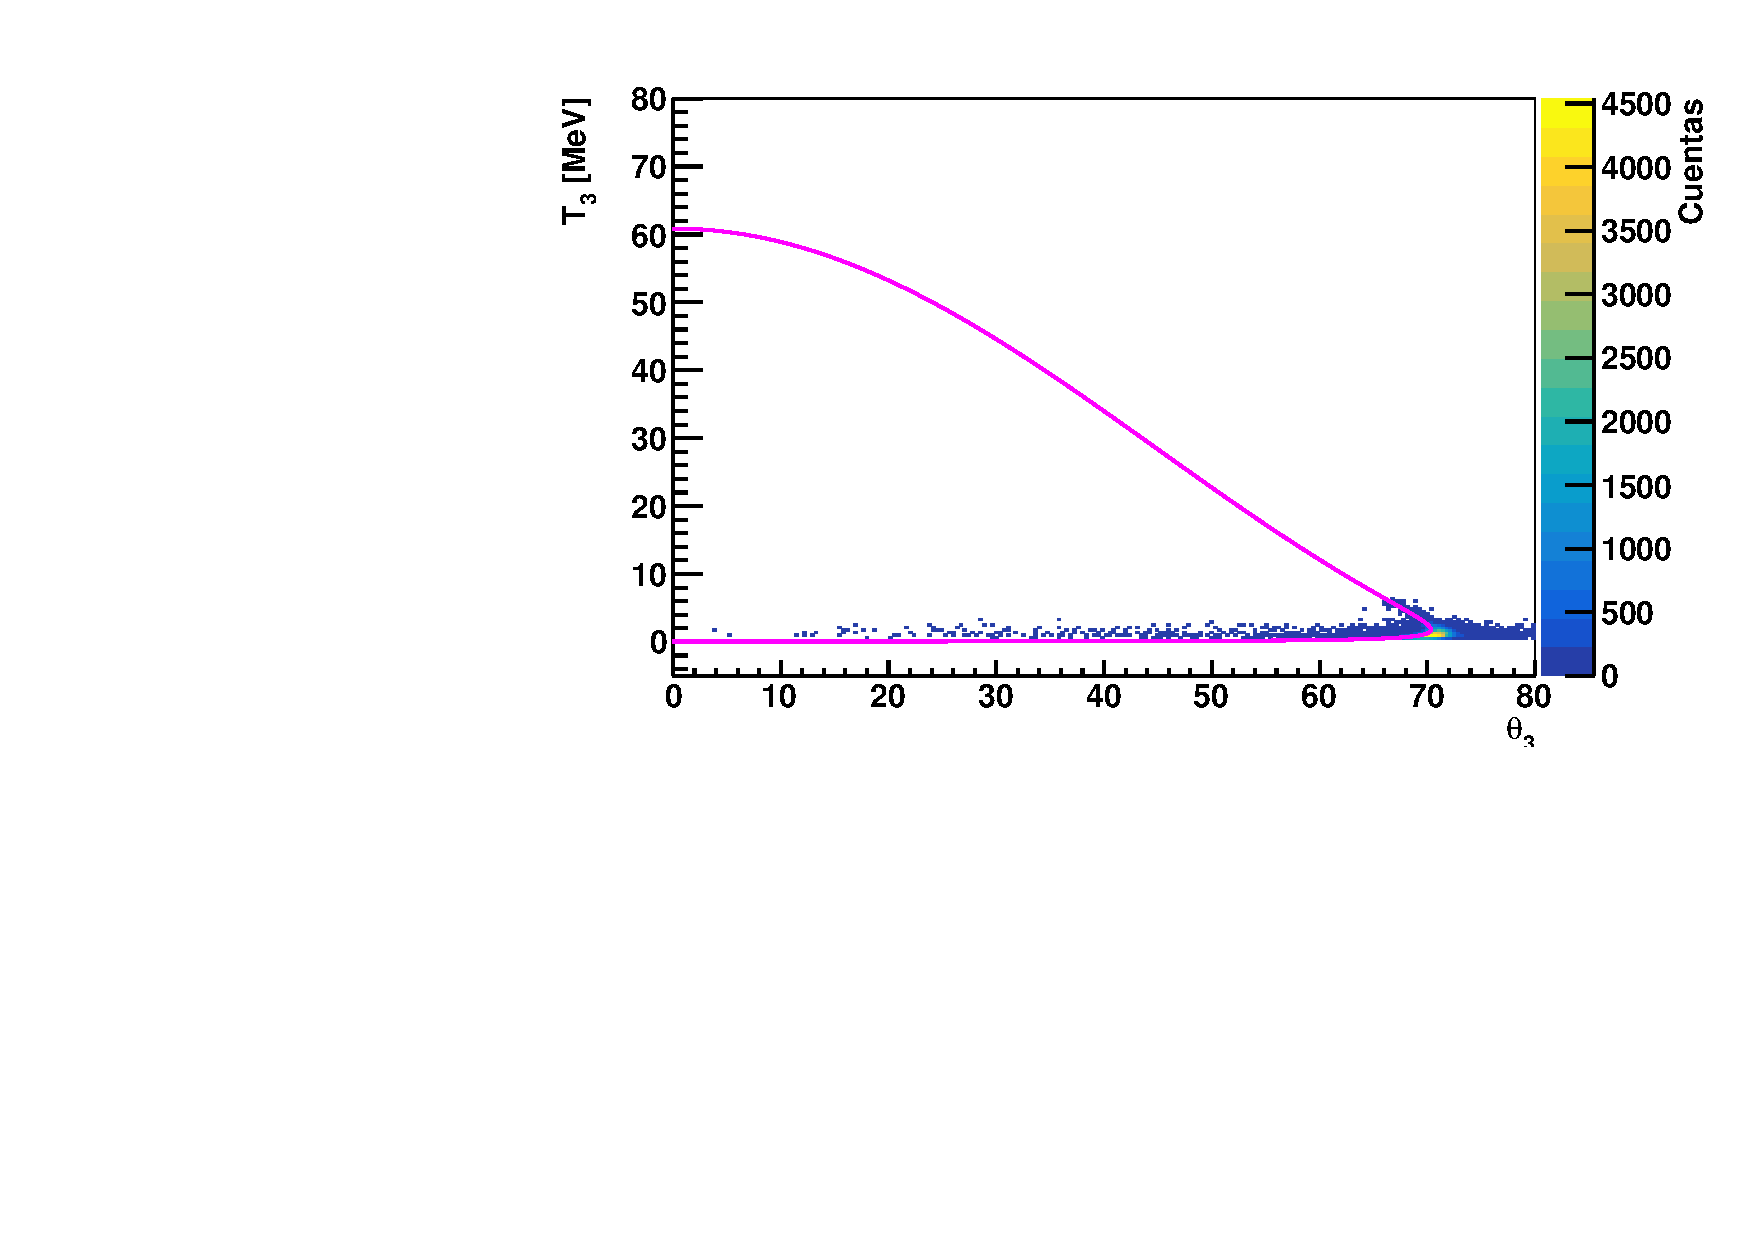
\includegraphics[width=0.6\linewidth]{Imagenes/Trigger/EkinMeasuredL1_Ex0.00_incIdx0.pdf}
    \caption{Cinemática de los eventos que se frenan en la cámara de deriva con todas las fuentes de incertidumbre y $E_x=0$ MeV.}
\end{figure}



Sin embargo no todas las partículas nos servirán para poder recostruir la cinemática, ya que los \textit{pads} tinene una resolución que no permite obtener conclusiones con aquellas partículas que tengan un \textit{punch-trought} menor que 20 mm. De todas las partículas que se paran podemos obtener un gran porcentaje de ellas, tal que: 

\begin{figure}[H] \centering
    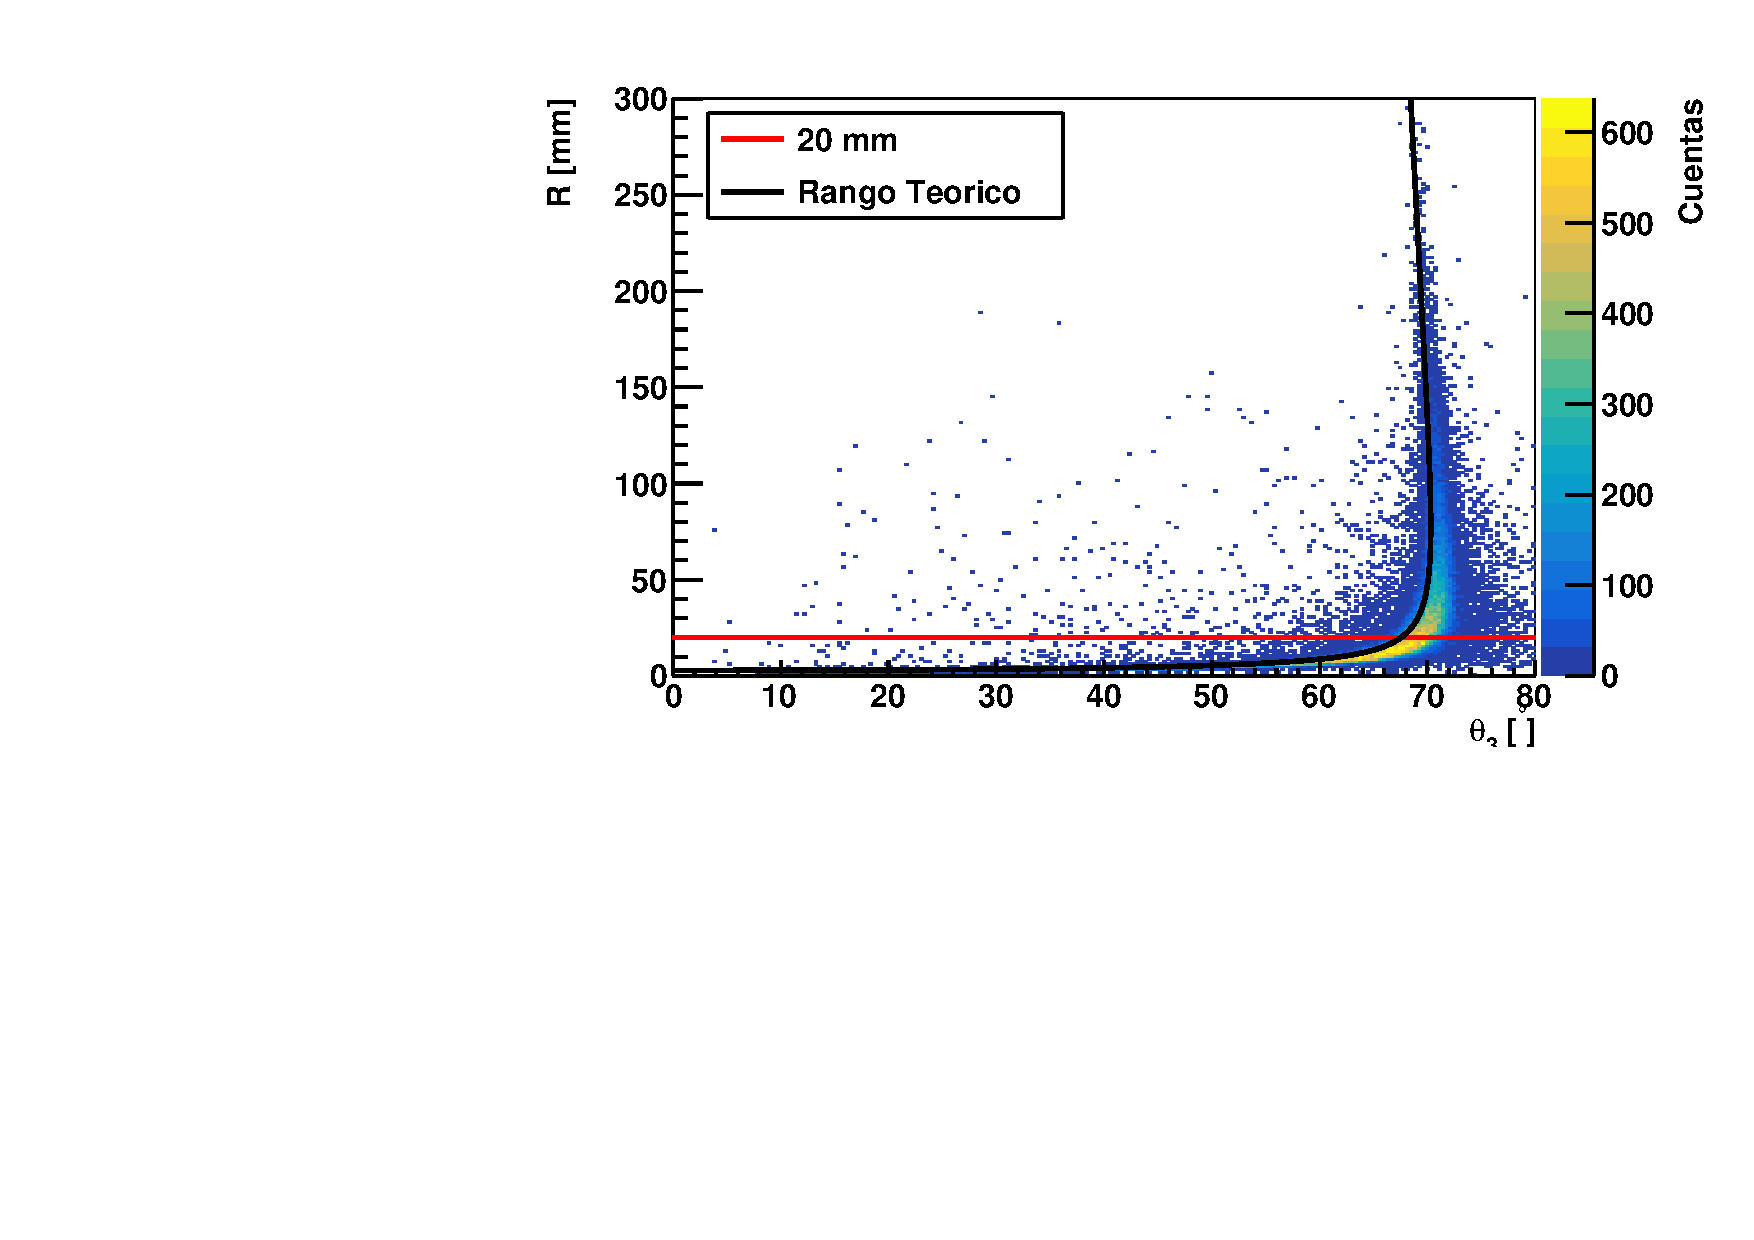
\includegraphics[width=0.6\linewidth]{Imagenes/Trigger/RangeTheta_Ex0.00_incIdx0.pdf}
    \caption{Cinemática de los eventos que se frenan en la cámara de deriva con todas las fuentes de incertidumbre y $E_x=0.0$ MeV.}
\end{figure}


Con el siguiente porcentaje de eventos rescuperales dentro de todos los que se paran (cocientre entre aquellos eventos con rango menor de 2 cm, tal que:

\begin{table}[H] \centering
    \begin{tabular}{llll} \hline
\toprule 
$E_{x}=0.0$ MeV & $E_{x}=0.20$ MeV \\ 
 \midrule 
 51.2438\% & 75.0016\% &\\ 
\bottomrule 
\end{tabular}
    
\end{table}